\section{Symmetric Alice and Bob}
\textit{In this exercise, the flows between Alice and Bob are symmetric, similar to the discussions in class, meaning that each source provides a throughput of R to the system. This means that the system load at any point will be 2R. The task is to give derive the analytical expressions for the throughput for the case of not using network coding and the case of using network coding in the presence of a Medium Access Control (MAC) mechanism that provides fair access to the channel. Assume no losses occur in the different communication channels.}

\subsection{Exercise 1: Throughput Without Network Coding}
\textit{It is recommended to attack this problem in three stages. First, identify the three key regions of operation when not using network coding justifying your answer. Second, derive analytical expressions for the total system throughput, i.e., the addition of the end-to-end throughput of the connection from Alice to Bob and from Bob to Alice, versus the system load (2R). Finally, plot the total system throughput versus the system load.}\\

In the case without network coding the Relay has to send the data of Alice and Bob independently, so the data packets dispatched will be 2 times the packets sent by one of them.  This situation will end when the maximum capacity is reached, in which limit the throughput is 0.5 R with a $25\%$ of the load system, where A and B are sending $R/4$. \\
After this point the nodes Alice and Bob will inject more packets, overloading the system and causing a drop of the throughput as they're stealing the capacity to the relay, which has to discard the rest. When the overload reach the point in which each node and the Relay have the same capacity ($33%$) the system is balanced and the rest of the packets from Alice and Bob will be discarded before entering the system. After this point the throughput will stay stable at that value. To have a better understanding a plot (\figref{fig:throughput_NC}) of the throughput vs the load of the system is made.
\begin{figure}[!h]
  \centering
  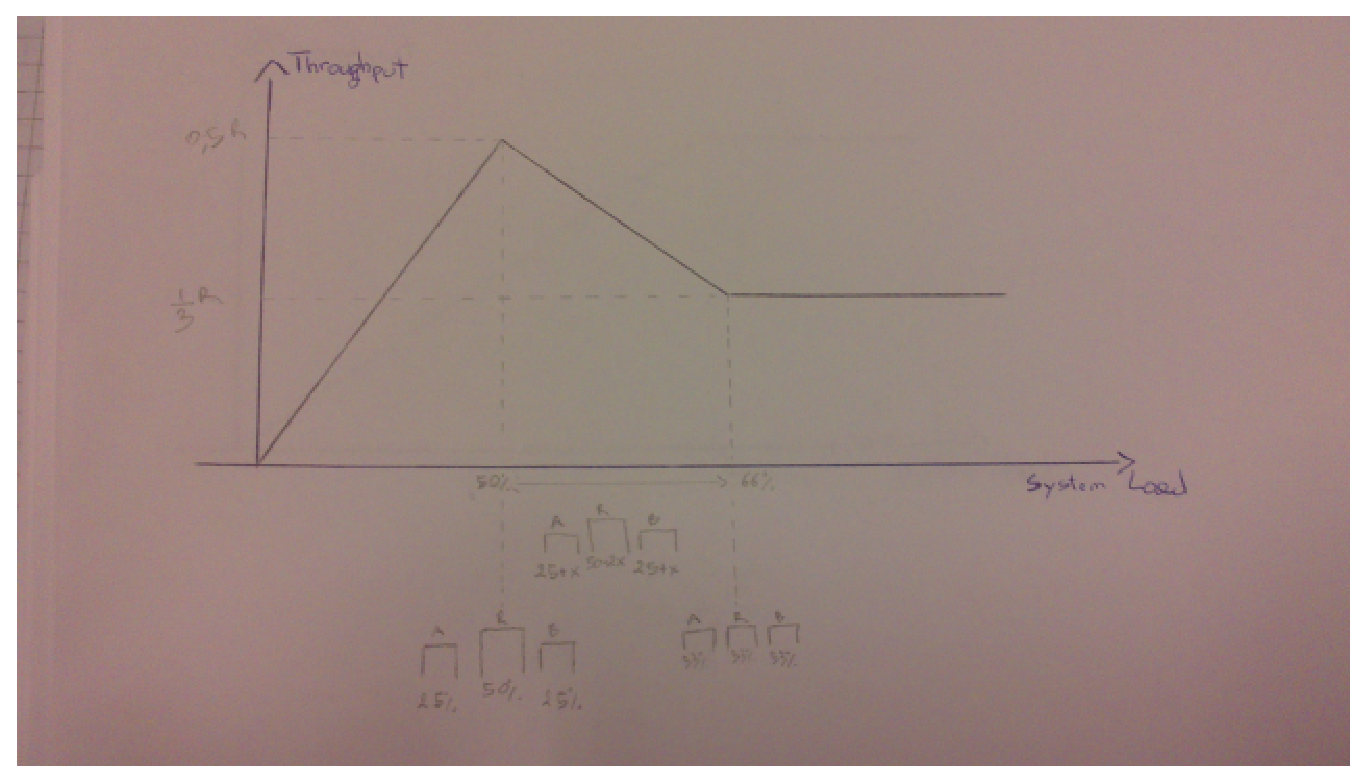
\includegraphics[width=13cm]{throughput_NC.eps}
  \caption{throughput without NC}
  \label{fig:throughput_NC}
\end{figure}
\newpage
\subsection{Exercise 2: Throughput With Network Coding}
\textit{Repeat the steps of the previous question but using inter-session network coding at the relay. How many regions of operations are there and why?}\\

For the Network Coding the scenario is a bit different. The relay in this case can combine the packet from Alice and from Bob in one coded packet The throughput will grow until the maximum capacity is reached ($\dfrac{2}{3} R $), since each node is able to send $R/3$ without any packet being discarded and it will stay stable with a $66 \%$ of the system load. The \figref{fig:throughput_WNC} shows the situation described above.
\begin{figure}[!h]
  \centering
  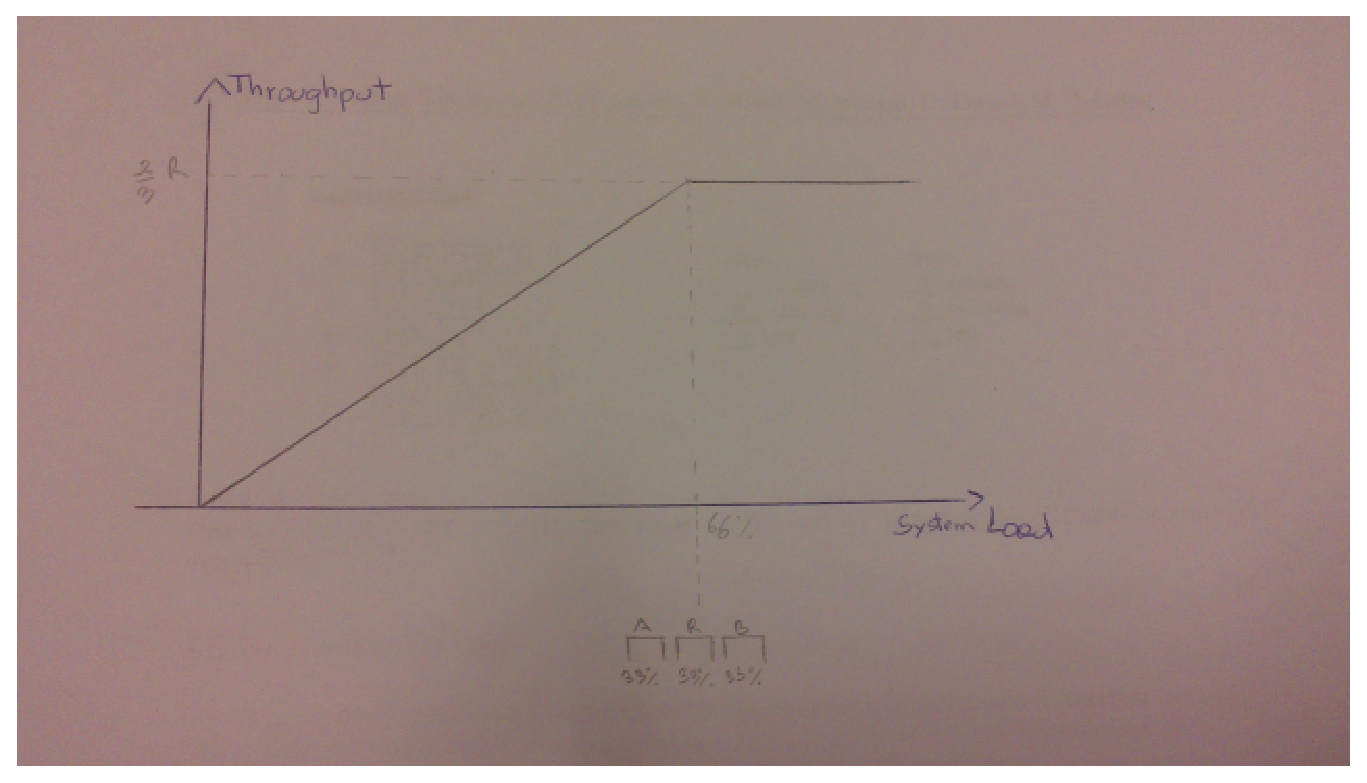
\includegraphics[width=13cm]{throughput_WNC.eps}
  \caption{throughput with NC}
  \label{fig:throughput_WNC}
\end{figure}
